\documentclass[../main.tex]{subfiles}
\usepackage{slashed}
\usepackage[table]{xcolor}
\usepackage{hhline}
\usepackage{lipsum}

\let\Bbbk\relax
\usepackage{amsmath}
\usepackage{amsfonts}
\usepackage{simpler-wick}


\begin{document}
\setchapterimage[6.5cm]{images_ch3/...}
\setchapterpreamble[u]{\margintoc}
\chapter[???]{???\footnotemark[0]}
\labch{???}
\fboxsep =1pt % separazione per i box

\section{Divergenze Infrarosse}
Lo studio delle divergenze infrarosse richiederebbe un corso a parte, in questa sezione vogliamo dare semplicemente alcune utili nozioni basilari.

Abbiamo già incontrato questo tipo di divergenze nel calcolo della derivata dell'auto-energia del fotone nell'esercizio \ref{ex:dSigma_dpslashed}, così come anche nel calcolo del fattore di forma elettrico al loop in $q^2=0$, nell'esercizio \ref{ex:1loop_formfactor1}, e abbiamo visto che possono essere regolarizzate a patto dell'inserimento di una massa del fotone fittizia.

\subsection{Scattering Coulombiano al tree-level}
\marginnote{\[\feynmandiagram[horizontal'=a to b, inline=(a.base)] {
    i1 -- [anti fermion, edge label=\(p'\)] a[dot] -- [anti fermion, edge label=\(p\)] i2,
    b[large, crossed dot] -- [photon, momentum'=\(q\)] a
    };\]}
Studiamo nuovamente lo scattering Coulombiamo, di cui riportiamo la cinematica:
\[
\begin{aligned}
&p+q=p' \\
&E_p = E_{p'} \\\
&q^2=-|\Vec q|^2 = -2|\Vec p|^2\big(1-\cos\vartheta\big)
\end{aligned}
\Rightarrow
\begin{cases}
q = p' - p \\
|\Vec p| = |\Vec p'|\\
\boxed{q^2 = -4|\Vec p|^2 \sin^2\frac{\vartheta}{2}} 
\end{cases}
\]
Mentre per quanto riguarda l'ampiezza del processo al tree-level, abbiamo:
\[
\boxed{i\mathscr M_0  = (ie)\bar u (p',s)\gamma^0 u (p,r) \frac{Ze}{|\Vec{q}|^2}}
\]

Ne consegue che, ricordando quanto detto nella nota \ref{note:wick_contraction} in merito all'origine delle tracce e sfruttando le proprietà delle matrici $\gamma$:
\begin{align*}
    \frac{1}{2}\sum_{s,r}|\mathscr M_0|^2 &= \frac{Z^2e^4}{2|\Vec{q}|^4}\Tr{\big(\slashed p' + m\big)\gamma^0 \big(\slashed p + m\big)\gamma^0}\\
    &=\frac{Z^2e^4}{2|\Vec{q}|^4}4\big[2p^0p'^0 + m^2-p\cdot p'\big] \overset{\blacklozenge}{=}
\end{align*}
Adesso sostituiamo le condizioni cinematiche e semplifichiamo il semplificabile:

\begin{align*}
    \overset{\blacklozenge}{=}\frac{Z^2e^4}{8|\Vec p|^4 \sin^4\frac{\vartheta}{2}}\big[E^2 + m^2 + |\Vec{p}|^2 \cos\vartheta\big] 
\end{align*}
Si verifica che \(E^2 + m^2 + |\Vec{p}|^2 \cos\vartheta = 2E^2\big[ 1 - \beta^2\sin^2\frac{\vartheta}{2} \big]\) con \(\beta\equiv \frac{|\Vec{p}|}{E}\), quindi in definitiva:

\begin{align*}
\boxed{\frac{1}{2}\sum_{s,r}|\mathscr M_0|^2 = \frac{Z^2e^4}{4|\Vec p|^2\beta^2 \sin^4\frac{\vartheta}{2}}\bigg[ 1 - \beta^2\sin^2\frac{\vartheta}{2}\bigg]}
\end{align*}
Presa per nota la sezione d'urto differenziale \(\frac{d\sigma}{d\Omega}=\frac{1}{(4\pi)^2}\times \frac{1}{2}\sum_{s,r}|\mathscr M_0|^2\), abbiamo in questo caso:
\[
\frac{d\sigma}{d\Omega}= \frac{1}{2}\sum_{s,r}|\mathscr M_0|^2 = \frac{Z^2\alpha^2}{4|\Vec p|^2\beta^2 \sin^4\frac{\vartheta}{2}}\bigg[ 1 - \beta^2\sin^2\frac{\vartheta}{2}\bigg]
\]

\subsection{Correzioni al vertice}
Includiamo adesso le correzioni al vertice, studiando nuovamente il diagramma:
\marginnote{\(V\) sta ad identificare la presenza di un fotone Virtuale, e l'indice $\mu$ sarà contratto con la carica esterna che, come specificato nel seguito, al momento non abbiamo interesse a considerare.}
\[
\begin{tikzpicture}[baseline=\plusheight]
    \begin{feynman}
    \vertex (i) at (-2,1) {};
    \vertex[small, dot] (x) at (-1,0.5) {};
    \vertex[small, dot] (v) at (0,0) {};
    \vertex[small, dot] (y) at (1,0.5) {};
    \vertex (f) at (2,1) {};
    \vertex[large, crossed dot] (N) at (0,-1) {};
    \diagram*[small]{
    (i) --[fermion, edge label'=\(p\)] (x) --[fermion, edge label'=\(p-k\)] (v) --[fermion, edge label'=\(p'-k\)] (y) --[fermion, edge label'=\(p'\)] (f),
    (x) --[photon, half left, looseness=0.8, momentum=\(k\)](y),
    (N) --[photon] (v)
    };
    \end{feynman}
\end{tikzpicture} = i\mathscr M^\mu_V
\]
Abbiamo già studiato questo diagramma in precedenza, e abbiamo anche visto quanto fosse complesso il calcolo della sua ampiezza, da cui emergeva una divergenza infrarossa. 

L'idea è quella di svolgere nuovamente il calcolo di tale ampiezza, \textbf{tralasciando il potenziale generato dal nucleo}, utilizzando una serie di approssimazioni ad-hoc, utili ad isolare fin dal principio il termine divergente nel regime infrarosso.

In maniera preliminare scriviamo:
\begin{align*}
    i\mathscr M^\mu_V = i(ie^3)\int\frac{d^4k}{(2\pi)^4}\frac{1}{k^2+i\epsilon}\frac{\bar u(p')\gamma^\rho\big(\slashed p'-\slashed k + m\big)\gamma^\mu\big(\slashed p-\slashed k + m\big)\gamma_\rho u(p)}{\big[(p'^2-k)^2 -m^2 + i\epsilon\big]\big[(p^2-k)^2 -m^2 + i\epsilon\big]}
\end{align*}
$\blacktriangleright$ Siccome le divergenze IR appaiono nel limite \(\boxed{k\rightarrow0}\), questa sarà la nostra prima semplificazione: trascuriamo \(k\) al numeratore e \(k^2\) al denominatore; inoltre prendiamo i fermioni sulla shell di massa.
\begin{align*}
    i\mathscr M^\mu_V \overset{\text{IR}}{=} i(ie^3)\int\frac{d^4k}{(2\pi)^4}\frac{1}{k^2+i\epsilon}\frac{\bar u(p')\gamma^\rho\big(\slashed p' + m\big)\gamma^\mu\big(\slashed p+ m\big)\gamma_\rho u(p)}{\big[-2k\cdot p' + i\epsilon\big]\big[-2k\cdot p + i\epsilon\big]}
\end{align*}
$\blacktriangleright$ Ora semplifichiamo il numeratore per mezzo dell'equazione di Dirac:
\[
\begin{aligned}
    &\bar u(p') \big(\slashed p' - m\big) = 0  \\
    &\big(\slashed p - m\big)u(p) = 0
\end{aligned}
\Rightarrow
\begin{cases}
    \bar u(p') \slashed p' = \bar u(p')m \\
    \slashed p u(p)  =  m u(p)
\end{cases}
\]
Ma per farlo dobbiamo “girare” i prodotti \(\gamma^\rho \slashed p'\) e \(\slashed p\gamma_\rho\) sfruttando le relazioni di anticommutazione tra le gamma di Dirac \(\big[\gamma^\rho, \gamma^\mu\big]_+ = 2g^{\rho\mu}\).
\marginnote{
A titolo di esempio riportiamo l'operazione citata nel caso di $p'$:
\begin{align*}
    \gamma^\rho \slashed p' &= \gamma^\rho \gamma^\mu p'_\mu = (-\gamma^\mu\gamma^\rho + 2g^{\rho\mu})p'_\mu =\\
    &=-\slashed p'\gamma^\rho + 2p'^\rho 
\end{align*}}

Applicando questa operazione ed utilizzando successivamente \textcolor{blue}{l'equazione di Dirac} otteniamo:
\begin{align*}
    \mathscr N^\mu &= \bar u(p')\big(\Ccancel[blue]{-\slashed p'\gamma^\rho} + 2p'^\rho + \Ccancel[blue]{m\gamma^\rho}\big)\gamma^\mu\big(\Ccancel[blue]{-\gamma_\rho\slashed p} + 2p_\rho+ \Ccancel[blue]{\gamma_\rho m}\big) u(p)\\
    &=4p'\cdot p\,\bar u(p')\gamma^\mu u(p)
\end{align*}

Arriviamo quindi al seguente risultato

\begin{equation}
    \boxed{
    \begin{aligned}
        i\mathscr M^\mu_V \overset{\text{IR}}{=}&
        \bar u(p')\big(ie\gamma^\mu\big)u(p)\big(ie\big)^2 4ip'\cdot p\,\times \\
        &\times\int\frac{d^4k}{(2\pi)^4}\frac{1}{\big(k^2+i\epsilon\big)\big(2k\cdot p'-i\epsilon\big)\big(2k\cdot p-i\epsilon\big)}
    \end{aligned}}
    \label{eq:IR_factorized_coulomb_amplitude}
\end{equation}
Ci accorgiamo quindi del fatto che, nel limite infrarosso \(k\rightarrow0\), \textbf{la correzione virtuale} (dovuta allo scambio di un fotone virtuale tra le gambe esterne) \textbf{fattorizza nell'ampiezza al tree-level per un integrale IR-divergente}.

Diagrammaticamente: \marginnote{Notiamo come in questo passaggio il fattore 4 venga semplificato raccogliendo un 2 in ciascuna delle due parentesi a denominatore.}
\[
\boxed{
\begin{aligned}
    &\begin{tikzpicture}[baseline=\plusheight]
        \begin{feynman}
        \vertex (i) at (-1.5,1) {};
        \vertex[small, dot, Red] (x) at (-0.75,0.5) {};
        \vertex[small, dot, Red] (v) at (0,0) {};
        \vertex[small, dot, Red] (y) at (0.75,0.5) {};
        \vertex (f) at (1.5,1) {};
        \vertex (N) at (0,-1) {};
        \diagram*[small,Red]{
        (i) --[fermion, edge label'=\(p\)] (x) -- (v) -- (y) --[fermion, edge label'=\(p'\)] (f),
        (x) --[photon, half left, looseness=0.8](y),
        (N) --[photon] (v)
        };
        \end{feynman}
    \end{tikzpicture}\overset{\text{IR}}{=}
    \begin{tikzpicture}[baseline=\plusheight]
        \begin{feynman}
        \vertex (i) at (-1.5,1) {};
        \vertex[dot, Green] (v) at (0,0) {};
        \vertex (f) at (1.5,1) {};
        \vertex (N) at (0,-1) {};
        \diagram*[small,Green]{
        (i) --[fermion, edge label'=\(p\)] (v) --[fermion, edge label'=\(p'\)] (f),
        (N) --[photon] (v)
        };
        \end{feynman}
    \end{tikzpicture} \times \textcolor{blue}{\text{ Integrale IR-divergente}}\\
    &\textcolor{Red}{\mathscr M^\mu_V}\quad \overset{\text{IR}}{=}\quad \textcolor{Green}{\mathscr M_0^\mu} \quad\times\quad\textcolor{blue}{(-i)e^2 p\cdot p'\int\frac{d^4k}{(2\pi)^4}\frac{1}{\big(k^2+i\epsilon\big)\big(k\cdot p'-i\epsilon\big)\big(k\cdot p-i\epsilon\big)}}
\end{aligned}}
\]

Concentriamoci a questo punto sull'integrale su \(k\) e separiamo l'integrazione spaziale da quella temporale:
\[
\int\frac{d^3\Vec k}{(2\pi)^3}\int\limits_{-\infty}^{+\infty}\frac{d k^0}{(2\pi)}\frac{1}{\big[(k^0)^2-|\Vec{k}|^2+i\epsilon\big]}\frac{1}{\big(k^0p'^0 -\Vec{k}\cdot\Vec p' -i\epsilon\big)\big(k^0p^0 -\Vec{k}\cdot\Vec p-i\epsilon\big)} \overset{\star}{=}
\]
Consideriamo quindi i poli nel piano complesso di \(k^0\), e ci accorgiamo che tre dei poli si trovano sopra l'asse reale:
\marginnote{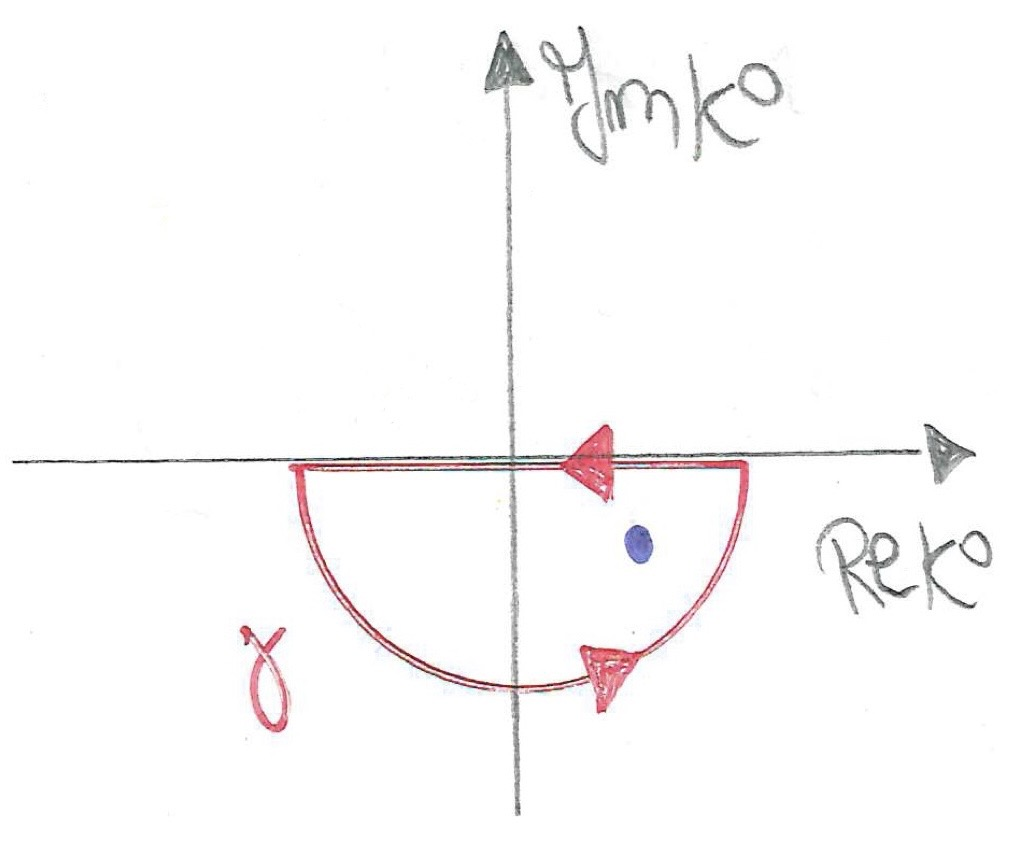
\includegraphics[]{images_ch5/k0_integration_contour.jpg}}
\[
k^0 =
\begin{cases}
      |\Vec{k}| - i\varepsilon\\ 
      -|\Vec{k}| + i\varepsilon
\end{cases} \quad , \quad
\begin{cases}
    k^0 = \frac{\Vec{k}\cdot\Vec p'}{p'^0} + i\varepsilon\\ \\
    k^0 = \frac{\Vec{k}\cdot\Vec p}{p^0} + i\varepsilon
\end{cases}
\]

Per comodità integriamo su una circonferenza nella parte inferiore del piano complesso come mostrato a lato, in modo da includere solo il polo \(k^0_\ast = |\Vec{k}| - i\varepsilon\).

Svolgendo il calcolo applicando il teorema dei residui e successivamente passando in coordinate polari modificando la misura di integrazione \(d^3\Vec k \rightarrow |\Vec{k}|^2 d|\Vec{k}|d\Omega\), otteniamo:

\[
\text{\marginnote{Ricordiamo che dal teorema dei residui, $\gamma$ come in figura, abbiamo (con il “$-$” per via del verso di integrazione):
\[\int_\gamma f(k^0) = - 2\pi i \text{Res}(f,k^0_\ast) \]
dove, per poli semplici come quello considerato:
\[
\text{Res}(f,k^0_\ast) = \lim_{k^0\rightarrow k^0_\ast}\big(k^0- k^0_\ast\big) f(k^0)
\]}}
\begin{aligned}
   &\overset{\star}{=}-i\int\frac{d^3\Vec k}{(2\pi)^3}\frac{1}{2|\Vec{k}|}\frac{1}{|\Vec{k}|^2\big(p'^0 -|\Vec{p}'| \cos\vartheta_{kp'}\big)\big(p^0 -|\Vec{p}| \cos\vartheta_{kp}\big)}\\
   &=-i \int\frac{\Ccancel[blue]{|\Vec{k}|^2} d|\Vec{k}|d\Omega}{(2\pi)^3 2|\Vec{k}|}\frac{1}{\Ccancel[blue]{|\Vec{k}|^2}\big(p'^0 -|\Vec{p}'| \cos\vartheta_{kp'}\big)\big(p^0 -|\Vec{p}| \cos\vartheta_{kp}\big)}
\end{aligned}
\]

In definitiva abbiamo l'espressione finale per la correzione virtuale:

\begin{equation}
    \boxed{
   \mathscr M^\mu_V \overset{\text{IR}}{=}\mathscr M_0^\mu
   \frac{(-e^2) p\cdot p'}{16\pi^3}\int \frac{d|\Vec{k}|}{|\Vec{k}|}\frac{d\Omega}{\big(p'^0 -|\Vec{p}'| \cos\vartheta_{kp'}\big)\big(p^0 -|\Vec{p}| \cos\vartheta_{kp}\big)}
   }
   \label{eq:IR_factorized_coulomb_amplitude_final}
\end{equation}
Questa ampiezza è, parlando in termini di power-counting, logaritmicamente divergente nel limite \(|\Vec{k}|\rightarrow 0\) (che corrisponde al limite \(\lambda \rightarrow\infty\)). Divergenze di questo tipo sono note come \textbf{divergenze infrarosse soft} o singolarità di massa (in quanto connesse alla presenza di particelle massless nello spettro).

\begin{nota}
    Consideriamo la parte angolare dell'integrale: i fattori \(\big(p'^0 -|\Vec{p}'| \cos\vartheta_{kp'}\big)\) e \(\big(p^0 -|\Vec{p}| \cos\vartheta_{kp}\big)\) non si annullano mai finché si considera l'elettrone come massivo.

    In realtà, se ci pensiamo su, in QED sono anche sempre strettamente positivi!
    Infatti la richiesta \(\big(p^0 -|\Vec{p}| \cos\vartheta_{kp}<0\) richiederebbe 
    \[
    \cos\vartheta_{kp}>\frac{p^0}{|\Vec{p}|}
    \]
    ma l'energia dell'elettrone, a causa della sua massa, è sempre maggiore del modulo del suo impulso, seppure di poco, i.e.: \(\frac{p^0}{|\Vec{p}|} > 1\).

    Di conseguenza la condizione richiesta non può essere soddisfatta in alcun caso, e diciamo che \textbf{in QED con elettroni massivi sono presenti solo divergenze infrarosse soft legate al fotone massless}.
    \label{note:softIRdiv_are_related_to_photons_only}
\end{nota}
\begin{nota}
    Supponiamo per un attimo gli elettroni come particelle massless, i.e. \(p^0=|\Vec{p}|,~ p'^0=|\Vec{p'}|\). 

    In questo caso la funzione nell'integrale angolare diventa
    \[
    \frac{1}{|\Vec{p'}|\big(1- \cos\vartheta_{kp'}\big)|\Vec{p}|\big(1- \cos\vartheta_{kp}\big)}
    \]
    È evidente che questa funzione presenti divergenze nel limite \(\vartheta_{kp}\rightarrow 0\) oppure \(\vartheta_{kp'}\rightarrow 0\).

    Anche queste sono divergenze infrarosse, questa volta associate alla non-massività dell'elettrone, e sono dette \textbf{divergenze infrarosse collineari}. Ovviamente in massive-QED non avremo mai a che fare con questo tipo di divergenze, ma la situazione è diversa se si considerano altre teorie, come ad esempio la QCD.
    \label{note:collinear_IR_divergences}
\end{nota}

\subsection{Diagramma di emissione reale}
Fino ad ora abbiamo ragionato in termini di scattering Coulombiano, tuttavia il risultato che abbiamo ottenuto è piuttosto generale.

Consideriamo infatti il processo:
\[
e^-(p) + X \rightarrow e^-(p')+X
\]
che schematizziamo al tree-level (al solito indicato con il pedice “$0$”) come segue:
\[
\begin{tikzpicture}[baseline=\plusheight]
        \begin{feynman}
        \vertex (i) at (-1.5,1) {};
        \vertex[dot, fill=white!100, minimum size=7mm] (v) at (0,0) {\(iB\)};
        \vertex (f) at (1.5,1) {};
        \diagram*[small]{
        (i) --[fermion, edge label'=\(p\)] (v) --[fermion, edge label'=\(p'\)] (f),
        };
        \end{feynman}
    \end{tikzpicture}  \equiv i\mathscr M_0 = \bar u(p')iB u(p)
\]
dove \(iB\) rappresenta una generica interazione, ad esempio quella con una carica esterna nel caso dello scattering Coulombiano.

La sezione d'urto per questo processo sarà:
\[
\boxed{\sigma_0(e^-X\rightarrow e^-X) = \frac{1}{2\mathscr I}\int\sum_{s,r} |\mathscr M_0|^2d\Phi_{e^-X}}
\]
dove indichiamo con \(\mathscr I\) il flusso iniziale di elettroni e con \(d\Phi_{e^-X}\) l'elemento di spazio delle fasi su cui stiamo integrando per quanto riguarda lo stato finale.

Se adesso includiamo le correzioni al loop nella nostra trattazione e ripetiamo il calcolo fatto nel caso dello scattering Coulombiano, trascurando i termini di ordine \(k^2\) che emergono nei denominatori dei propagatori interni e semplificando il numeratore sfruttando l'equazione di Dirac, arriviamo anche in questo caso ad una fattorizzazione del tipo “ampiezza al tree-level $\times$ integrale IR-divergente”:

\[
\begin{tikzpicture}[baseline=\plusheight]
    \begin{feynman}
    \vertex (i) at (-1.5,1) {};
    \vertex[small, dot] (x) at (-0.75,0.5) {};
    \vertex[dot, fill=white!100, minimum size=7mm] (v) at (0,0) {\(iB\)};
    \vertex[small, dot] (y) at (0.75,0.5) {};
    \vertex (f) at (1.5,1) {};
    \vertex (N) at (0,-1) {};
    \diagram*[small]{
    (i) --[fermion, edge label'=\(p\)] (x) -- (v) -- (y) --[fermion, edge label'=\(p'\)] (f),
    (x) --[photon, half left, looseness=0.8](y),
    };
    \end{feynman}
\end{tikzpicture} = i\mathscr M_V \overset{\text{IR}}{=} i\mathscr M_0 \times \substack{\text{integrale} \\ \text{IR-divergente}}
\]

Il che ha senso se pensiamo al fatto che fotoni con lunghezze d'onda molto grandi sicuramente non saranno sensibili a processi di scattering che si svolgono a piccole scale, come il processo al tree-level.

Ora portiamo la discussione su questioni pratiche: il fatto che quest'ampiezza sia divergente è un bel problema. Infatti non c'è contro-termine che regga per regolarizzare questa divergenza, tutta la libertà che avevamo nel giocare con i parametri della teoria si è esaurita quando abbiamo rimosso le divergenze ultraviolette.

Nel momento in cui andiamo a calcolare la sezione d'urto ad un loop, fermandoci al prim'ordine in teoria delle perturbazioni (i.e. trascurando termini di ordine pari o superiore a \(|\mathscr M|^2\)), troviamo:
\begin{align*}
    \sigma_1(e^-X\rightarrow e^-X) &= \frac{1}{2\mathscr I}\int\sum_{s,r} |\mathscr M_0 + \mathscr M_V|^2 d\Phi_{e^-X}\\
    & = \frac{1}{2\mathscr I}\int\sum_{s,r}\Big[|\mathscr M_0|^2 + \mathscr M_0^\ast \mathscr M_V + \mathscr M_V^\ast \mathscr M_0\Big]\\
    & = \frac{1}{2\mathscr I}\int\sum_{s,r}|\mathscr M_0|^2 d\Phi_{e^-X} + \frac{1}{2\mathscr I}\int\sum_{s,r}\Big[ \mathscr M_0^\ast \mathscr M_V + \mathscr M_V^\ast \mathscr M_0\Big] d\Phi_{e^-X}
\end{align*}

Nel primo integrale riconosciamo la sezione d'urto al tree-level e se semplifichiamo il secondo a dovere il risultato finale sarà:
\begin{equation}
    \boxed{
    \begin{aligned}
        \sigma_1(e^-X\rightarrow e^-X) = ~
        &\sigma_0(e^-X\rightarrow e^-X) ~\times\\
        & \bigg[1 - \frac{e^2p\cdot p'}{8\pi^3}\int \frac{d|\Vec{k}|}{|\Vec{k}|}\frac{d\Omega}{\big(p'^0 -|\Vec{p}'| \cos\vartheta_{kp'}\big)\big(p^0 -|\Vec{p}| \cos\vartheta_{kp}\big)}\bigg]
    \end{aligned}
    }
    \label{eq:1loop_virtual_cross_section}
\end{equation}
Anche la sezione d'urto diverge nel limite infrarosso! Come facciamo ad eliminare queste divergenze senza usare i contro-termini?

L'idea è quella di considerare lo stesso processo includendo un fotone extra nello stato finale. Al tree-level questo significa considerare i diagrammi:

\[
\begin{tikzpicture}[baseline=\plusheight]
    \begin{feynman}
    \vertex (i) at (-1.5,1) {\(p\)};
    \vertex[small, dot] (x) at (-0.75,0.5) {};
    \vertex (z) at (0,1) {};
    \vertex[dot, fill=white!100, minimum size=7mm] (v) at (0,0) {\(iB\)};
    \vertex (f) at (1.5,1) {\(p'\)};
    \diagram*[small]{
    (i) --[fermion] (x) --[fermion, edge label'=\(p-k\)] (v) --[fermion] (f),
    (x) --[photon, momentum=\(k\)] (z),
    };
    \end{feynman}
\end{tikzpicture}
+
\begin{tikzpicture}[baseline=\plusheight]
    \begin{feynman}
    \vertex (i) at (-1.5,1) {\(p\)};
    \vertex (z) at (0.75,1.5) {};
    \vertex[dot, fill=white!100, minimum size=7mm] (v) at (0,0) {\(iB\)};
    \vertex[small, dot] (y) at (0.75,0.5) {};
    \vertex (f) at (1.5,1) {\(p'\)};
    \diagram*[small]{
    (i) --[fermion] (v) --[fermion, edge label'=\(p'+k\)] (y) --[fermion] (f),
    (y) --[photon, momentum=\(k\)] (z),
    };
    \end{feynman}
\end{tikzpicture}
\]
Il ragionamento per cui introduciamo questi diagrammi nel nostro calcolo regge anche dal punto di vista fisico: essendo l'elettrone una particella carica accelerata, deve perdere energia per irraggiamento!

Consideriamo il primo diagramma, la sua ampiezza (con il pedice $R$ ad indicare l'emissione di un fotone “Reale” e non virtuale) sarà:

\begin{align*}
    i\mathscr M_R^{(1)} &= \bar u(p')iB \frac{i\big(\slashed p - \slashed k + m\big)}{\big(p-k\big)^2 -m^2 + i\epsilon}\big[ie\gamma^\mu\varepsilon_\mu^\ast(k)\big]u(p) \\
    &\overset{\text{IR}}{=}\bar u(p')iB \frac{i\big(\slashed p + m\big)}{-2p\cdot k + i\epsilon}\big(ie\gamma^\mu\big)u(p)\varepsilon_\mu^\ast(k)\tikzmark{a}\\
    &=\bar u(p')iB \frac{(-e)2p^\mu\varepsilon_\mu^\ast(k)}{-2p\cdot k + i\epsilon}u(p) \tikzmark{b}\\
    &=\big[\bar u(p')iB u(p)\big]\frac{(-e)2p^\mu\varepsilon_\mu^\ast(k)}{-2p\cdot k + i\epsilon}
\end{align*}
\sidecomment{a}{b}{a}{eq. di Dirac}
E con le stesse modalità si trova l'espressione per il secondo diagramma. 

In sintesi abbiamo:
\begin{align*}
    &i\mathscr M_R^{(1)} \overset{\text{IR}}{=} i\mathscr M_0\bigg[\frac{(-e)2p^\mu\varepsilon_\mu^\ast(k)}{-2p\cdot k + i\epsilon}\bigg]\\
    &i\mathscr M_R^{(2)} \overset{\text{IR}}{=} i\mathscr M_0\bigg[\frac{(-e)2p'^\mu\varepsilon_\mu^\ast(k)}{2p'\cdot k + i\epsilon}\bigg]
\end{align*}

Di conseguenza possiamo scrivere l'ampiezza totale al tree-level:
\begin{equation}
    \boxed{
    i\mathscr M_R \overset{\text{IR}}{=} i\mathscr M_0\bigg[-e
    \underbrace{\bigg(\frac{2p'^\mu}{2p'\cdot k + i\epsilon} -\frac{2p^\mu}{2p\cdot k - i\epsilon}\bigg)}_{\substack{\text{fattori di emissione}\\\text{per un fotone soft}}}
    \bigg]}
    \label{eq:total_treelevel_amplitude_realemission}
\end{equation}

Non ci resta che calcolare la sezione d'urto, sommando su spin e polarizzazione dei fotoni nello stato finale e integrando sullo spazio delle fasi a tre corpi, ovvero:
\[
\sigma(e^-X\rightarrow e^-X+\gamma) = \frac{1}{2\mathscr I}\int\sum_{\text{spin}} |\mathscr M_0|^2d\Phi_{e^-X\gamma}
\]

Il risultato che otteniamo è il seguente:
\begin{equation}
    \boxed{
    \begin{aligned}
        \sigma(e^-X\rightarrow e^-X\gamma) \overset{\text{IR}}{=} ~
        &\sigma_0(e^-X\rightarrow e^-X) \sum_\text{elicità}\int \frac{d^3\Vec{k}}{(2\pi)^3 2E_k}e^2\Bigg\{ \\
        & \bigg(\frac{p'^\mu}{p'\cdot k}-\frac{p^\mu}{p\cdot k} \bigg) \varepsilon_\mu^\ast(k)\varepsilon_\nu(k) \bigg(\frac{p'^\nu}{p'\cdot k}-\frac{p^\nu}{p\cdot k}\bigg)\Bigg\}
    \end{aligned}
    }
    \label{eq:cross_section_total_realemission}
\end{equation}
Notiamo quindi due cose:
\begin{enumerate}
    \item[\textbf{i)}] Nel limite infrarosso lo spazio delle fasi fattorizza; infatti la parte che si riferisce allo stato finale \(e^-X\) insieme al flusso iniziale e al modulo quadro dell'ampiezza al tree-level ricostruiscono \(\sigma_0(e^-X\rightarrow e^-X)\).
    
    \item[\textbf{ii)}] La parte che descrive l'emissione del fotone genera invece un integrale su \(\Vec k\), sommato sulle polarizzazioni fisiche del fotone stesso.
\end{enumerate}
Concentriamoci sull'integrale di emissione: ricordando l'equazione (\ref{eq:polsum_final}) possiamo sostituire la somma sulle elicità dei vettori di polarizzazione con un tensore metrico con segno negativo, i.e. \(-g_{\mu\nu}\) (i termini aggiuntivi, come ampiamente discusso, sono irrilevanti). Gli indici degli impulsi sono quindi tutti uguali e possiamo svolgere i prodotti, ottenendo:
\[
-e^2\int \frac{d^3\Vec{k}}{(2\pi)^3 2|\Vec{k}|}\bigg[\frac{p'^2}{(p'\cdot k)^2} + \frac{p^2}{(p\cdot k)^2} -\frac{2p'\cdot p}{(p\cdot k)(p'\cdot k)}\bigg]
\]

Concentriamoci sul terzo termine, in quanto gli altri due vengono magicamente cancellati dal contro-termine \(\delta_2\).

Svolgiamo quindi il prodotto al denominatore e passiamo in coordinate polari:

\begin{align*}
    \frac{e^2(p\cdot p')}{8\pi^3}\int \frac{d|\Vec{k}|}{|\Vec{k}|}|\Vec{k}|^2d\Omega \frac{1}{|\Vec{k}|^2(p'^0-|\Vec{p}|\cos\vartheta_{kp'})(p^0-|\Vec{p'}|\cos\vartheta_{kp})}
\end{align*}
Questo integrale ci risulta piuttosto familiare. In effetti è esattamente identico a quello che appare nella sezione d'urto che abbiamo trovato studiando il diagramma con il fotone virtuale tra le gambe esterne, i.e. quella in equazione (\ref{eq:1loop_virtual_cross_section})!

Ciò significa che, fidandoci del fatto che gli altri due termini si cancellino per i motivi di cui sopra, \textbf{la somma delle due sezioni d'urto}
\[
\boxed{\sigma_1(e^-X\rightarrow e^-X) + \sigma(e^-X\rightarrow e^-X\gamma)}
\]
\textbf{non diverge nel limite infrarosso}, i.e. è \textit{IR-finite}.

\begin{nota}
    Rimarchiamo i due concetti chiave appena appresi in termini leggermente diversi:
    \begin{enumerate}
        \item[\textbf{1)}] Le sezioni d'urto \textbf{esclusive}, i.e. del tipo \(\sigma(e^-X\rightarrow e^-X)\), soffrono delle divergenze infrarosse e non sono quantità osservabili.
        \item[\textbf{2)}] Le sezioni d'urto \textbf{inclusive}, i.e. del tipo \(\sigma(e^-X\rightarrow e^-X +\gamma 's)\), sono libere dalle divergenze infrarosse.
    \end{enumerate}
    \label{note:exclusive/inclusive_xsec_remarks}
\end{nota}

Ragioniamo ora dal punto di vista sperimentale:
in quale senso \(\sigma(e^-X\rightarrow e^-X)\), come rimarcato nella nota \ref{note:exclusive/inclusive_xsec_remarks}, non è una quantità fisicamente osservabile? E perché dovremmo includere fotoni extra?

In un esperimento realistico, non avremo mai a disposizione un detector talmente sensibile da rivelare un fotone con energia \(E_\gamma\) piccola a piacere; difatti, dobbiamo sempre tener conto di una soglia \(\omega_\text{thr} \leftrightarrow E_\text{thr}\) sotto la quale questo detector non vede nulla.

Seguendo questa logica, appare evidente come lo stato finale \(|e^-X\gamma\rangle\), nel momento in cui \(E_\gamma < E_\text{thr}\), venga “visto” dal detector semplicemente come lo stato \(|e^-X\rangle\).

In altre parole, \textbf{le sezioni d'urto fisicamente misurabili devono includere ogni possibile numero di fotoni di bassa energia non rivelabili}. Riassumendo in formule:
\[
\boxed{\sigma(e^-X\rightarrow e^-X)_\text{obs} = \sigma(e^-X\rightarrow e^-X) + \sigma(e^-X\rightarrow e^-X+\gamma_{E_\gamma < E_\text{thr}})}
\]

Illustriamo a questo punto come avviene il processo di cancellazione delle divergenze. 
Partiamo dalla sezione d'urto esclusiva, i.e. l'equazione (\ref{eq:1loop_virtual_cross_section}), che può essere approssimata con le modalità che abbiamo già incontrato, introducendo la massa fittizia del fotone come regolatore per la divergenza infrarossa:
\[
\sigma_1(e^-X\rightarrow e^-X) \approx \sigma_0(e^-X\rightarrow e^-X)~\times~\bigg[ 1-\frac{\alpha}{\pi} f_{IR}\log\frac{E_e}{m_\gamma}\bigg]
\]

D'altro canto possiamo fare la stessa cosa anche per la sezione d'urto inclusiva, i.e. l'equazione (\ref{eq:cross_section_total_realemission}), con una piccola differenza. Abbiamo infatti:
\[
\sigma(e^-X\rightarrow e^-X\gamma) \approx \sigma_0(e^-X\rightarrow e^-X)~\times~\frac{\alpha}{\pi} f_{IR}\log\frac{\omega_\text{thr}}{m_\gamma}
\]

Il gioco è fatto! Se consideriamo la somma tra la sezione d'urto inclusiva ed esclusiva, cioè quella osservabile, separando i logaritmi vediamo che il termine con la “massa” del fotone si cancella!

\begin{equation}
    \boxed{
    \sigma(e^-X\rightarrow e^-X)_\text{obs} = \sigma_0(e^-X\rightarrow e^-X)~\times~\bigg[ 1-\frac{\alpha}{\pi} f_{IR}\log\frac{E_e}{\omega_\text{thr}}\bigg]
    }
    \label{eq:explicit_observable_xsec}
\end{equation}
L'equazione (\ref{eq:explicit_observable_xsec}) è \textit{IR-finite} nel limite \(m_\gamma\rightarrow 0\) e dipende dalla soglia \(\omega_\text{thr}>0\) in un esperimento reale. 

\begin{nota}
    Un piccolo recap sulla cancellazione delle divergenze.
    \begin{enumerate}
        \item[\textbf{UV:}] Emergono perché integriamo su un loop ad energie molto elevate \textcolor{gray}{[i.e., distanze estremamente corte]}, il che presumibilmente ci porta ben oltre la validità di qualsivoglia teoria quantistica di campo. 

        Il problema viene risolto reinterpretando la teoria e sfruttando i parametri liberi per cancellare i termini divergenti, connettendo questi parametri con le quantità osservabili.\\
        
        \item[\textbf{IR:}] Qui siamo nel caso opposto. Queste divegenze, infatti, appaiono quando si considera il limite di energia estremamente piccola \textcolor{gray}{[i.e., distanza estremamente grande]}. 
        
        Per correggere questo problema ridefiniamo le osservabili stesse, in quanto divergenze di questo tipo sono connesse a qualcosa che un esperimento realistico non sarà mai in grado di osservare.
    \end{enumerate}
\end{nota}

\begin{exercise}
    Nello studiare l'integrale di emissione abbiamo trascurato due dei tre termini che emergono nello sviluppo dell'espressione esplicita, i.e.: 
    \[
    -e^2\int \frac{d^3\Vec{k}}{(2\pi)^3 2|\Vec{k}|}\bigg[\underbrace{\frac{p'^2}{(p'\cdot k)^2} + \frac{p^2}{(p\cdot k)^2}}_{(\star)} -\frac{2p'\cdot p}{(p\cdot k)(p'\cdot k)}\bigg]
    \]
    Calcolare i contributi dei termini \((\star)\). Divergono nel limite infrarosso?
    [\textbf{conti svolti Lezione 18 pag. 80÷82}]
\end{exercise}

\end{document}